\documentclass[11pt]{article}
\usepackage[margin=1in]{geometry} 
\usepackage{amsmath,amsthm,amssymb,amsfonts}
\usepackage{listings}
\usepackage{graphicx}
 
\newcommand{\N}{\mathbb{N}}
\newcommand{\Z}{\mathbb{Z}}

\newenvironment{problem}[2][Problem]{\begin{trivlist}
\item[\hskip \labelsep {\bfseries #1}\hskip \labelsep {\bfseries #2.}]}{\end{trivlist}}

\begin{document}
\title{CSE 574 Homework 1}
\author{Zackary Crosley}
\maketitle

\begin{problem}{1}
	Two dice are rolled
	\item Two dice are rolled simultaneously.
	\begin{itemize}
		\item Event A: The sum of two dice is 3.
		\item Event B: The sum of two dice is 7.
		\item Event C: At least one of the dice is 2.
	\end{itemize}
	
	\begin{enumerate}
		\item Compute P(A$|$C)
		
		\begin{equation}
			P(A|C) = \frac{P(C|A) \times P(A)}{P(C}
		\end{equation}
		\begin{equation}
			P(A|C) = \frac{1 \times P(A)}{P(C)}
		\end{equation}
		\begin{equation}
			P(A|C) = \frac{\frac{2}{36}}{1-\frac{5}{6} \times \frac{5}{6}}
		\end{equation}
		\begin{center}
			\textbf{P(A$|$C) = $\frac{2}{11}$}
		\end{center}
		\item Compute P(B$|$C)
		\begin{equation}
			P(B|C) = \frac{P(C|B) \times P(B)}{P(C)}
		\end{equation}
		\begin{equation}
			P(B|C) = \frac{\frac{2}{6} \times P(B)}{P(C)}
		\end{equation}
		\begin{equation}
			P(B|C) = \frac{\frac{2}{6} \times \frac{6}{36}}{1-\left(\frac{5}{6} \times \frac{5}{6} \right)} = \frac{\frac{2}{6} \times \frac{1}{6}}{1 - \frac{25}{36}}
		\end{equation}
		\begin{equation}
			P(B|C) = \frac{\frac{2}{36}}{\frac{11}{36}}
		\end{equation}
		\begin{center}
			\textbf{P(B$|$C) = $\frac{2}{11}$}
		\end{center}
	\end{enumerate}
\end{problem}

\begin{problem}{2}
	
	To win a chess tournament you must win two of three rounds in a row. Show that the optimal strategy is to play the weakest opponent second and the order of the other two doesn't matter.\newline
	\begin{verse}
	W$_i$ indicate winning a game against player i and L$_i$ indicate losing againt player i. Therefore in order to win the tournament one of the following conditions must be met:
	\end{verse}
	\begin{equation}
		\{W_1, W_2, W_3\}, \{W_1, W_2, L_3\}, \{L_1, W_2, W_3\}
	\end{equation}
	\begin{equation}
		P(\{W_1,W_2,W_3\}) = p_1 \times p_2 \times p_3
	\end{equation}
	\begin{equation}
		P(\{W_1,W_2,L_3\}) = p_1 \times p_2 \times (1 - p_3)
	\end{equation}
	\begin{equation}
		P(\{L_1,W_2,W_3\}) = (1 - p_1) \times p_2 \times p_3
	\end{equation}
	\begin{equation}
		P(\{W_1,W_2,W_3\} \lor \{L_1,W_2,W_3\} \lor \{W_1,W_2,L_3\}) = (p_1 \times p_2 \times p_3) + ((1 - p_1) \times p_2 \times p_3) + (p_1 \times p_2 \times (1 - p_3))
	\end{equation}
	\begin{equation}
		P(\{W_1,W_2,W_3\} \lor \{L_1,W_2,W_3\} \lor \{W_1,W_2,L_3\}) = p_2 \times (p_1 \times p_3 + (1 - p_1) \times p_3) + p_1 \times (1 - p_3))
	\end{equation}
	\begin{equation}
		P(\{W_1,W_2,W_3\} \lor \{L_1,W_2,W_3\} \lor \{W_1,W_2,L_3\}) = p_2 \times (p_1 + p_3 - p_1 \times p_3)
	\end{equation}
	\begin{verse}
		By Communative Property of addition and multiplication, we see that swapping the values of p$_1$ and p$_3$ would have no change to the equation outcome. Therefore the order of play against players 1 and 3 don't matter.
	\end{verse}
	\begin{verse}
		Playing the game with the highest probability of success as the second game is only optimal if:
	\end{verse}
	\begin{equation}
		p_2 \times (p_1 + p_3 - p_1 \times p_3) \geq p_1 \times (p_2 + p_3 + p_2 \times p_3)
	\end{equation}
	\begin{equation}
		p_2 \times p_1 + p_2 \times p_3 - p_1 \times p_2 \times p_3 \geq p_1 \times p_2 + p_1 \times p_3 - p_1 \times p_2 \times p_3
	\end{equation}
	\begin{equation}
		p_2 \times p_3 \geq p_1 \times p_3
	\end{equation}
	\begin{verse}
		Since $p_2 \geq p_1$ by definition, $p_2 \times p_3 \geq p_1 \times p_3$ must be true. Therefore, p$_2$ is more optimal in the second position than p$_1$. This property holds true for p$_3$ as well since the placement of $p_1$ and $p_3$ were shown to be irrelevant relative to one another.
	\end{verse}
	\begin{verse}
		Therefore, $p_2$ should be the match with the highest probability of winning.
	\end{verse}
\end{problem}
\begin{problem}{3}
	The output of a factory is produced by three machines that produce 20%, 30%, and 50% of factory output respectively with 5%, 3%, and 1% defective item respectively. If an item is chosen at random and is found to be defective, what are the odds it is from the third machine.
	\begin{equation}
		P(M_3|Defect) = \frac{P(Defect|M_3) \times P(M_3)}{P(Defect)}
	\end{equation}
	\begin{equation}
		P(M_3|Defect) = \frac{P(Defect|M_3) \times P(M_3)}{P(M_3, Defect) + P(M_2, Defect) + P(M_1, Defect)}
	\end{equation}
	\begin{equation}
		P(M_3|Defect) = \frac{P(Defect|M_3) \times P(M_3)}{P(Defect|M_3) \times P(M_3) + P(Defect|M_2) \times P(M_2) + P(Defect|M_1) \times P(M_1)}
	\end{equation}
	\begin{equation}
		P(M_3|Defect) = \frac{0.01 \times 0.50}{0.01 \times 0.50 + 0.03 \times 0.30 + 0.05 \times 0.20}
	\end{equation}
	\begin{equation}
		P(M_3|Defect) = \frac{0.005}{0.005 + 0.009 + 0.010} = \frac{0.005}{0.024}
	\end{equation}
	\begin{center}
		\textbf{P(M$_3|$Defect) = 0.208}
	\end{center}
\end{problem}
\begin{problem}{4}
	What is the expected product of the value rolled on two fair dies?
	\begin{equation}
		E[U] = \sum_{u \in U} u \times P(U = u)
	\end{equation}
	\begin{equation}
		E[U] = \frac{1}{36}\sum_{i,j = 1}^{6} i \times j = \frac{1}{6} \sum_{i=1}^{6} \frac{1}{6} \sum_{j=1}^{6} i \times j
	\end{equation}
	\begin{center}
		\textbf{E[U] = 12.25}
	\end{center}
\end{problem}
\begin{problem}{5}
	What is the expected number of die rolls before getting a 6?
	\begin{equation}
		E[X] = \sum_{x \in X} x \times P(X)
	\end{equation}
	\begin{equation}
		E[X] = \sum_{x=1}^{\infty} x \times (1-p)^{x-1} \times p
	\end{equation}
	\begin{equation}
		E[X] = p \times \sum_{x=1}^{\infty} x \times (1-p)^{x-1}
	\end{equation}
	\begin{equation}
		E[X] = p \times \left( \sum_{x=1}^{\infty} (1-p)^{x-1} + \sum_{x=2}^{\infty} (1-p)^{x-1} + \sum_{x=3}^{\infty} (1-p)^{x-1} + \ldots \right)
	\end{equation}
	\begin{equation}
		E[X] = p \times \left( \sum_{x=1}^{\infty} (1-p)^{x-1} + \sum_{x=1}^{\infty} (1-p)^{x} + \sum_{x=1}^{\infty} (1-p)^{x+1} + \ldots \right)
	\end{equation}
	\begin{equation}
		E[X] = p \times \left( \sum_{x=1}^{\infty} (1-p)^{x-1} + \sum_{x=1}^{\infty} (1-p)^{x-1}\times(1-p) + \sum_{x=1}^{\infty} (1-p)^{x-1}(1-p)^2 + \ldots \right)
	\end{equation}
	\begin{equation}
		E[X] = p \times \left( \frac{1}{1-(1-p)} + \frac{1-p}{1-(1-p)}+ \frac{(1-p)^2}{1-(1-p)}+ \ldots \right)
	\end{equation}
	\begin{equation}
		E[X] = p \times \left( \frac{1}{p} + \frac{1-p}{p}+ \frac{(1-p)^2}{p}+ \ldots \right)
	\end{equation}
	\begin{equation}
		E[X] = 1 + 1-p + (1-p)^2 + \ldots
	\end{equation}
	\begin{equation}
		E[X] = \frac{1}{1-(1-p)} = \frac{1}{p}
	\end{equation}
	\begin{center}
		\textbf{E[X] = $\frac{1}{6}$}
	\end{center}
\end{problem}
\begin{problem}{6}
	Let X be a random variable with probability mass function:
	
	\[
		f(x) = 
		\begin{cases}
			\frac{x^2}{a},& x = -3, -2, -1, 0, 1, 2, 3\\
			0,& \text{otherwise}
		\end{cases}
	\]
	
	Compute the value of a and E(x).
	\begin{equation}
		\sum_{x \in X} f(x) = 1
	\end{equation}
	\begin{equation}
		\sum_{x \in [-3, -2, -1, 0, 1, 2, 3]} f(x) = 1
	\end{equation}
	\begin{equation}
		f(-3) + f(-2) + f(-1) + f(0) + f(1) + f(2) + f(3) = 1
	\end{equation}
	\begin{equation}
		\frac{\left(-3\right)^2}{a} + \frac{\left(-2\right)^2}{a} + \frac{\left(-1\right)^2}{a} + \frac{\left(0\right)^2}{a} + \frac{\left(1\right)^2}{a} + \frac{\left(2\right)^2}{a} + \frac{\left(3\right)^2}{a} = 1
	\end{equation}
	\begin{equation}
		\frac{9 + 4 + 1 + 0 + 1 + 4 + 9}{a} = \frac{28}{a} = 1		
	\end{equation}
	\begin{center}
		\textbf{a = 28}
	\end{center}
	\begin{equation}
		E(X) = \sum_{x \in X} x \times P(X = x)
	\end{equation}
	\begin{equation}
		E(X) = \sum_{x \in [-3, -2, -1, 0, 1, 2, 3]} f(x) \times \frac{1}{7}
	\end{equation}
	\begin{equation}
		E(X) = \frac{1}{7} \times \left(f(-3) + f(-2) + f(-1) + f(0) + f(1) + f(2) + f(3)\right)
	\end{equation}
	\begin{equation}
		E(X) = \frac{1}{7} \times 28 = \frac{28}{7} = 4
	\end{equation}
	\begin{center}
		\textbf{E(X) = 4}
	\end{center}
\end{problem}
\begin{problem}{7}
	Compute the algorithmic complexity of the following algorithm.

	\begin{lstlisting}
		int i,j,k = 0;
		for (i = n/2; i <= n; i++) // Repeats n - n/2 times, or n/2.
			for (j = 2; j <= n; j *= 2) // Repeats log_2(n) - 1 times.
				k += n/2; 
	\end{lstlisting}
	
	\begin{verse}
		Time Complexity is O($\frac{n}{2} \times \left(\left(\log_2 n\right) -1\right)$)
	\end{verse}
\end{problem}
\begin{problem}{8}
	Find O Complexity for the following recurrence.
	\begin{lstlisting}
		T(n) = 2T(n-1) + 1 w/ T(0) = 0
	\end{lstlisting}
	\begin{verse}
		Can be re-written as:
	\end{verse}
	\begin{lstlisting}
		int val, prev_val = 0;
		for(i = 1; i <= n; i++) {
			int new_val = 2 * prev_val + 1;
			prev_val = new_val;
			val += new_val;
	\end{lstlisting}
	\begin{verse}
		Therefore this recurrence is O(n)
	\end{verse}
\end{problem}
\begin{problem}{9}
	\begin{enumerate}
		\item Find eigenvalues an eigenvectors of A and A$^2$
		\newline		
		$A = \begin{bmatrix} -1 & 3 \\ 2 & 0 \end{bmatrix}$
		\text{and}
		$A^2 = \begin{bmatrix} 7 & -3 \\ -2 & 6 \end{bmatrix}$
		\begin{equation}
			0 = det\left(\begin{bmatrix} -1-\lambda & 3 \\ 2 & 0-\lambda \end{bmatrix}\right)
		\end{equation}
		\begin{equation}
			(-1-\lambda)(-\lambda) - (2 \times 3) = \lambda^2 + \lambda - 6 = 0
		\end{equation}
		\begin{equation}
			\lambda_1 = -3, \lambda_2 = 2		
		\end{equation}
		\begin{equation}
			\begin{bmatrix} -1-\lambda & 3 \\ 2 & 0-\lambda \end{bmatrix} \Rightarrow \begin{bmatrix} -1+3 & 3 \\ 2 & 0+3 \end{bmatrix} \Rightarrow \begin{bmatrix} 2 & 3 \\ 2 & 3 \end{bmatrix}
		\end{equation}
		\begin{equation}
			\begin{bmatrix} 2 & 3 \\ 2 & 3 \end{bmatrix} \cdot \vec{v_1} = 0
		\end{equation}
		\begin{equation}
			\vec{v_1} = \begin{bmatrix}
				3 \\ -2
			\end{bmatrix}
		\end{equation}
		\begin{equation}
			\begin{bmatrix} -1-\lambda & 3 \\ 2 & 0-\lambda \end{bmatrix} \Rightarrow \begin{bmatrix} -1-2 & 3 \\ 2 & 0-2 \end{bmatrix} \Rightarrow \begin{bmatrix} -3 & 3 \\ 2 & -2 \end{bmatrix}
		\end{equation}
		\begin{equation}
			\begin{bmatrix} -3 & 3 \\ 2 & -2 \end{bmatrix} \cdot \vec{v_2} = 0
		\end{equation}
		\begin{equation}
			\vec{v_2} = \begin{bmatrix}
			1 \\ 1
			\end{bmatrix}
		\end{equation}
		\newline
		\begin{equation}
			0 = det\left(\begin{bmatrix} 7-\lambda & -3 \\ -2 & 6-\lambda \end{bmatrix}\right)
		\end{equation}
		\begin{equation}
			(7-\lambda)(6-\lambda) - (-2 \times -3) = \lambda^2 - 13\lambda +36 = 0
		\end{equation}
		\begin{equation}
			\lambda_1 = 9, \lambda_2 = 4
		\end{equation}
		\begin{equation}
			\begin{bmatrix} 7-\lambda & -3 \\ -2 & 6-\lambda \end{bmatrix} \Rightarrow \begin{bmatrix} 7-9 & -3 \\ -2 & 6-9 \end{bmatrix} \Rightarrow \begin{bmatrix} -2 & -3 \\ -2 & -3 \end{bmatrix}
		\end{equation}
		\begin{equation}
			\begin{bmatrix} -2 & -3 \\ -2 & -3 \end{bmatrix} \cdot \vec{v_1} = 0
		\end{equation}
		\begin{equation}
			\vec{v_1} = \begin{bmatrix}
				3 \\ -2
			\end{bmatrix}
		\end{equation}
		\begin{equation}
			\begin{bmatrix} 7-\lambda & -3 \\ -2 & 6-\lambda \end{bmatrix} \Rightarrow \begin{bmatrix} 7-4 & -3 \\ -2 & 6-4 \end{bmatrix} \Rightarrow \begin{bmatrix} 3 & -3 \\ -2 & 2 \end{bmatrix}
		\end{equation}
		\begin{equation}
			\begin{bmatrix} 3 & -3 \\ -2 & 2 \end{bmatrix} \cdot \vec{v_2} = 0
		\end{equation}
		\begin{equation}
			\vec{v_2} = \begin{bmatrix}
			1 \\ 1
			\end{bmatrix}
		\end{equation}
	\item Derive a relationship between the eigenvalues and eigenvectors fo the corresponding powers of the matrix A.
		\begin{equation}A \cdot \vec{x} = \lambda \cdot \vec{x} \end{equation}
		\begin{equation}A \cdot A \cdot \vec{x} = A \cdot \lambda \cdot \vec{x} \end{equation}
		\begin{equation}A \cdot A \cdot \vec{x} = \lambda \cdot A \cdot \vec{x} \end{equation}
		\begin{equation}A \cdot A \cdot \vec{x} = \lambda \cdot \left( \lambda \cdot \vec{x}\right) \end{equation}
		\begin{equation}A^2 \cdot \vec{x} = \lambda^2 \cdot \vec{x} \end{equation}
		\begin{verse}
			Therefore the eigenvalues ($\lambda$) are squared while the eigenvectors ($\vec{x}$) remain the same.
		\end{verse}
	\end{enumerate}
\end{problem}
\begin{problem}{10}
	Consider a state space where the start state is number 1 and the successor function for state n returns two states, numbers 2n and 2n+1
	\begin{enumerate}
		\item Draw the portion of the state space for states 1 to 15.
			\begin{figure}
				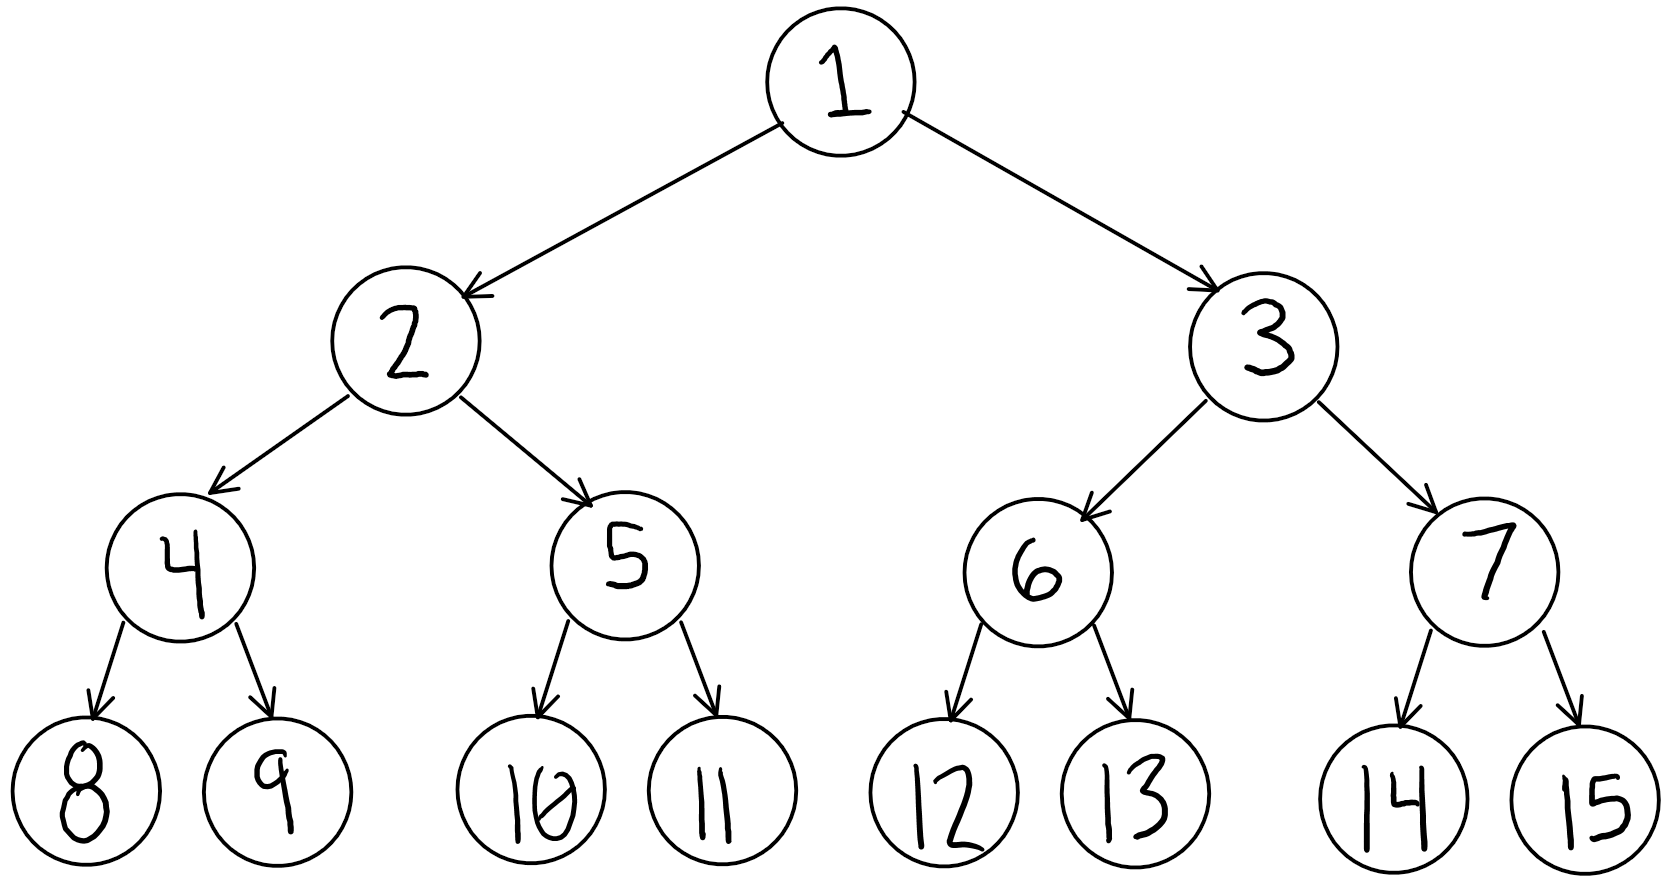
\includegraphics[scale=0.4]{TreeMain.PNG}
				\caption{State space for first 15 states.}
				\label{bfs.fig}
			\end{figure}					
		\item Suppose the goal state is 11. List the order in which nodes will be visited for a breadth first search, depth limited search with limit 3, and iterative deepening search.
			\newline
			\begin{large}Breadth First Search\end{large}
			\begin{figure}
				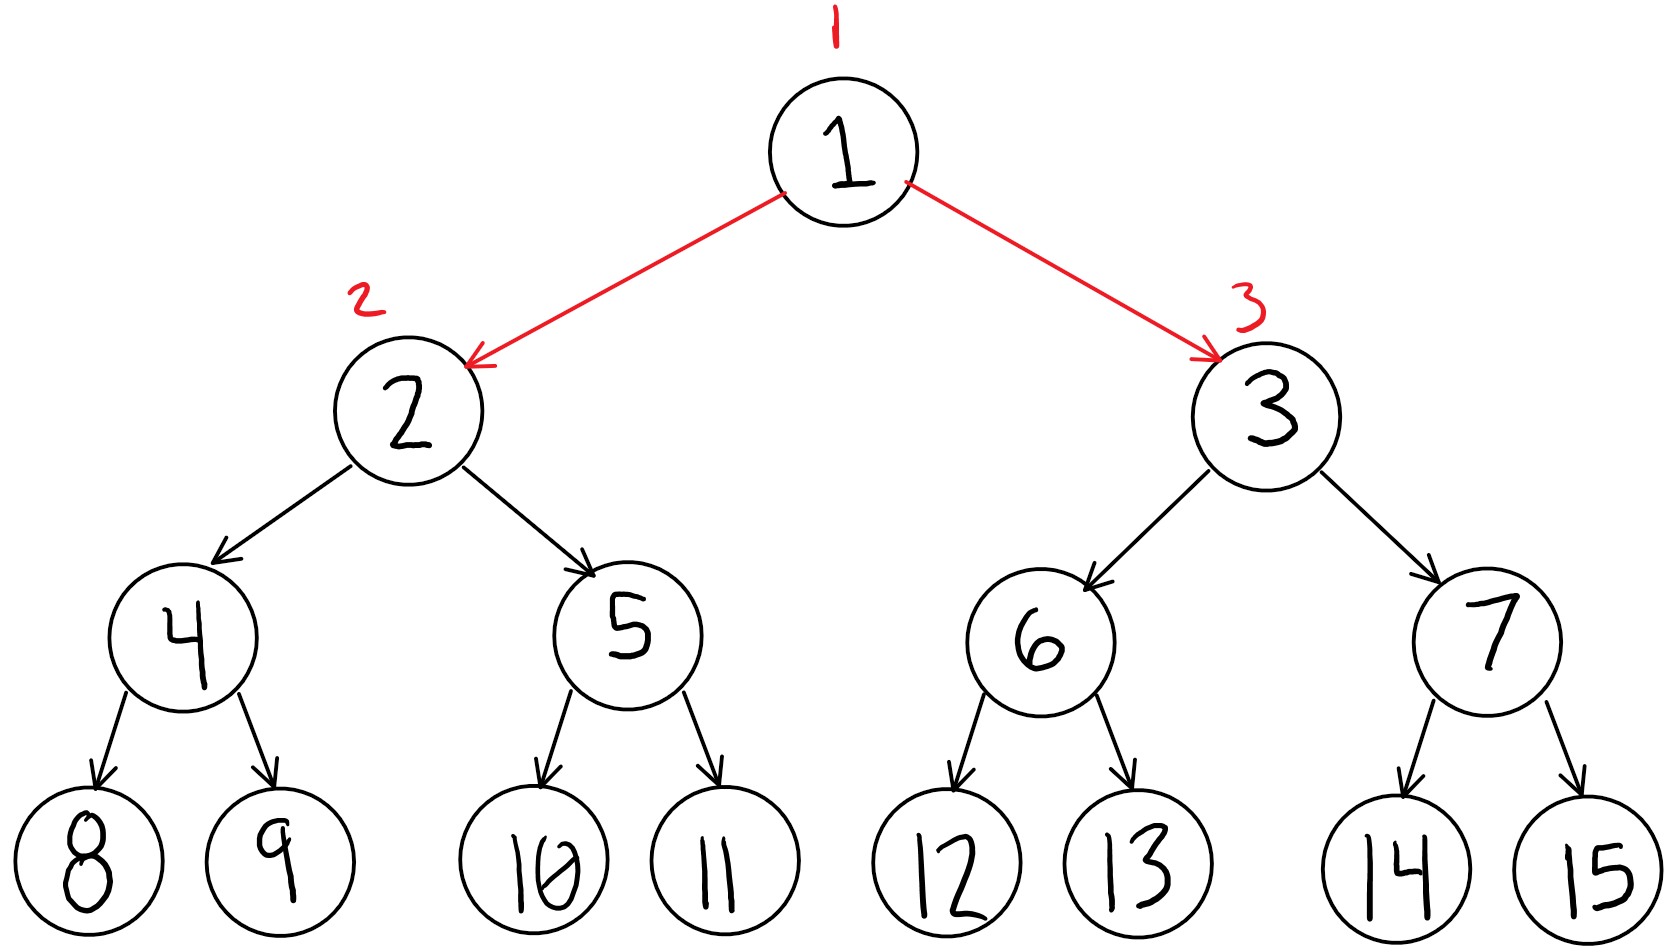
\includegraphics[scale=0.4]{BFS_1.png}
				\caption{First stage of Breadth First Search.}
				\label{fig.bfs}
			\end{figure}
			\begin{figure}
				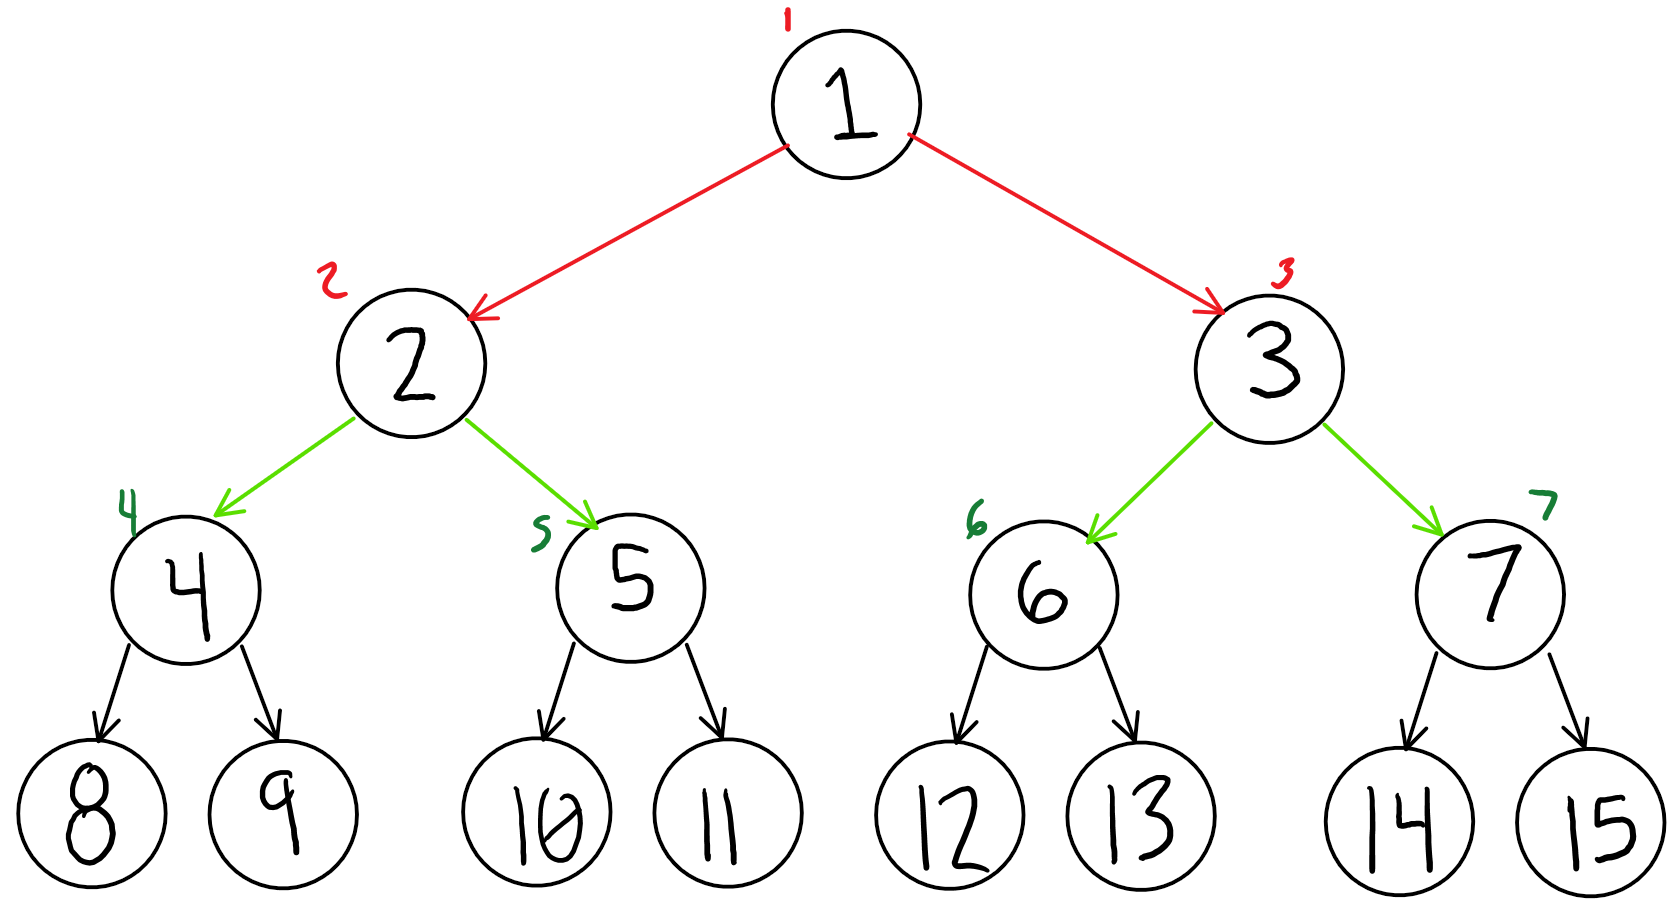
\includegraphics[scale=0.4]{BFS_2.PNG}
				\caption{Second stage of Breadth First Search.}
				\label{fig.bfs}
			\end{figure}
			\begin{figure}
				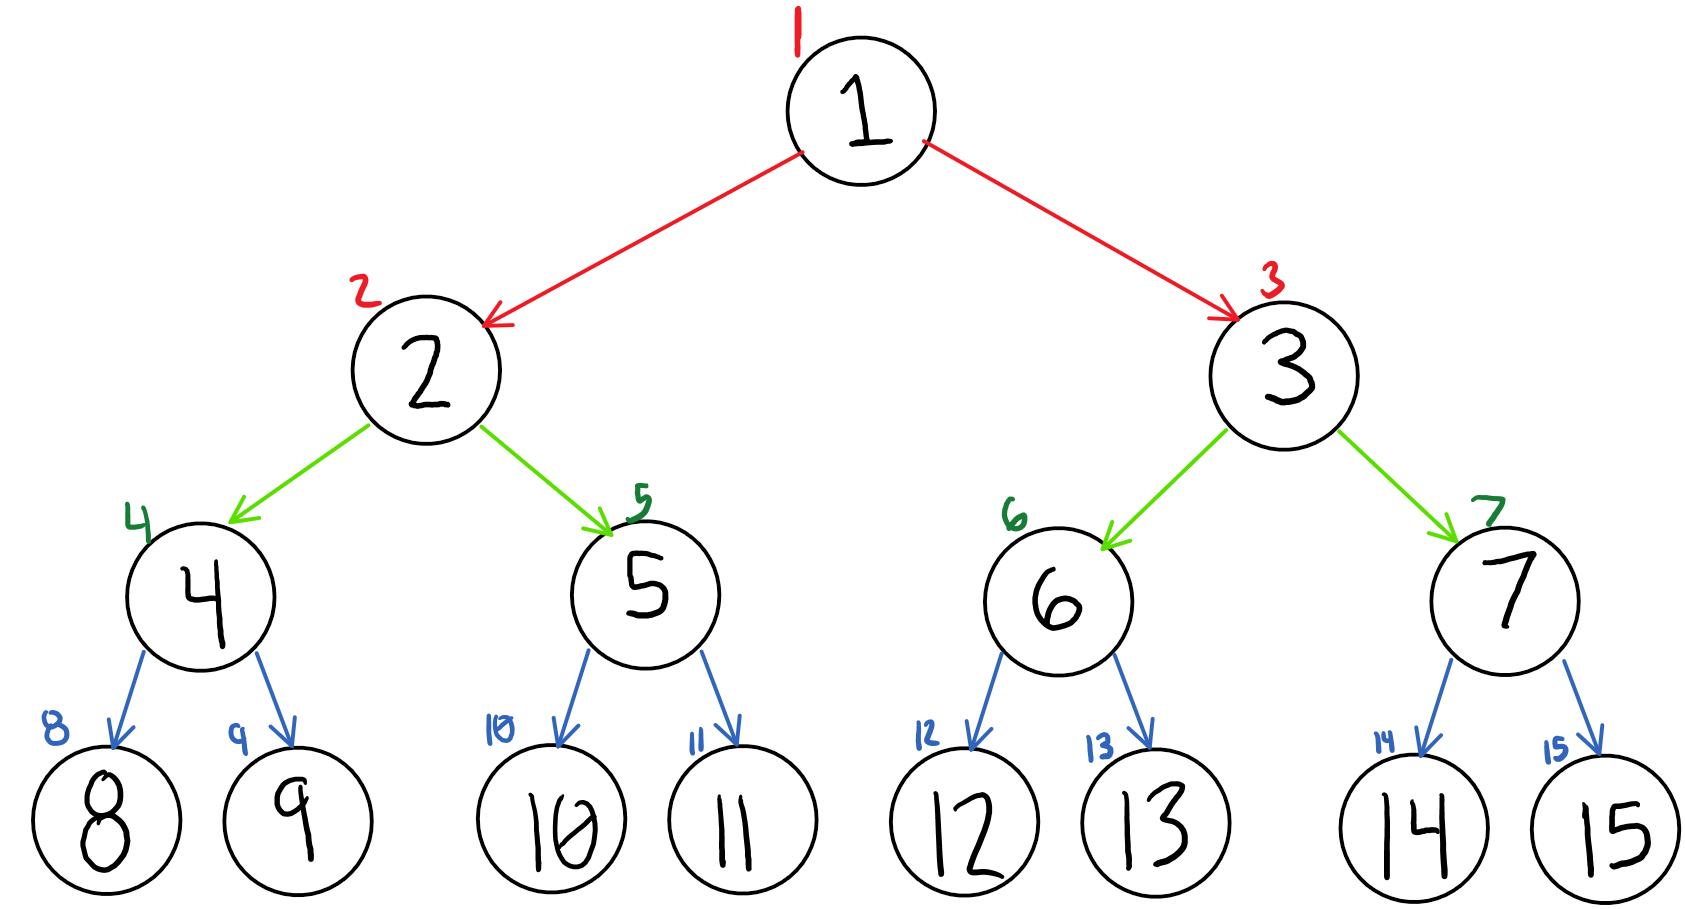
\includegraphics[scale=0.4]{BFS_3.PNG}
				\caption{Third stage of Breadth First Search.}
				\label{fig.bfs}
			\end{figure}
			\newline
			\begin{large}Depth Limited Search\end{large}
			\begin{figure}
				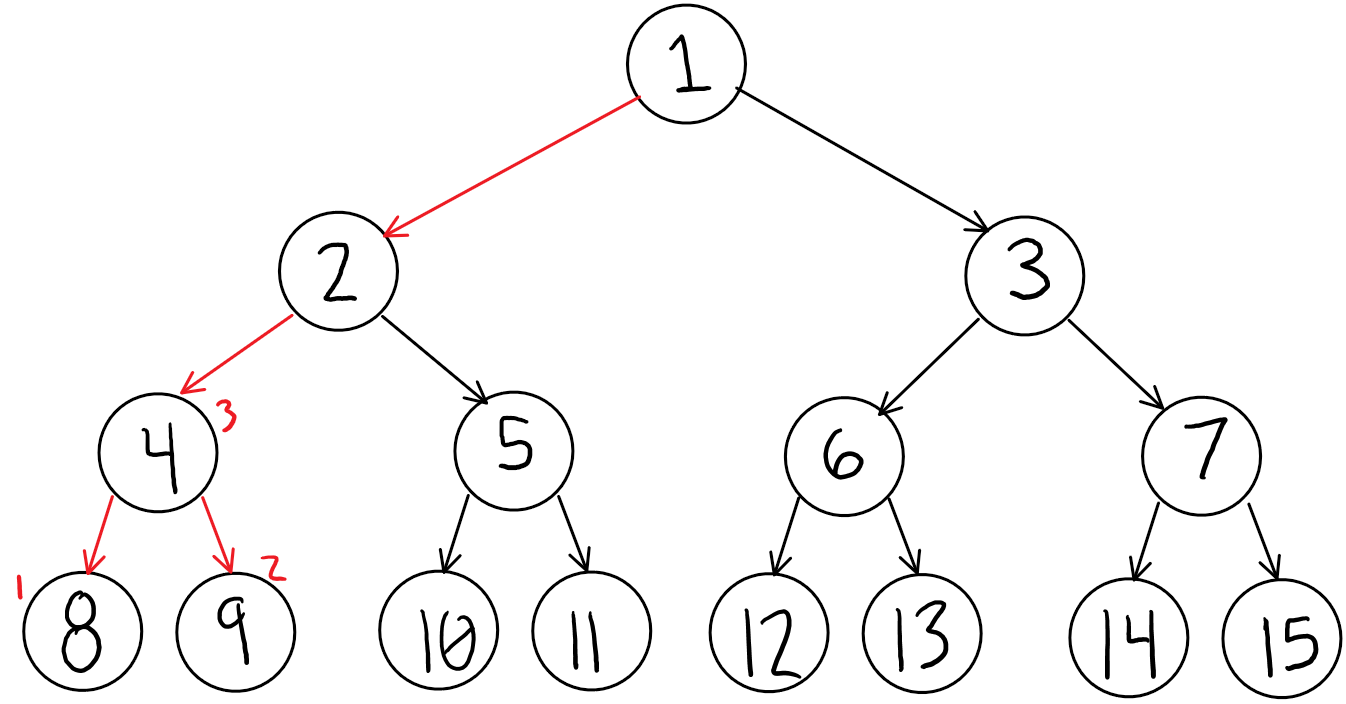
\includegraphics[scale=0.5]{DLS_1.png}
				\caption{First stage of Depth Limited Search.}
				\label{fig.bfs}
			\end{figure}
			\begin{figure}
				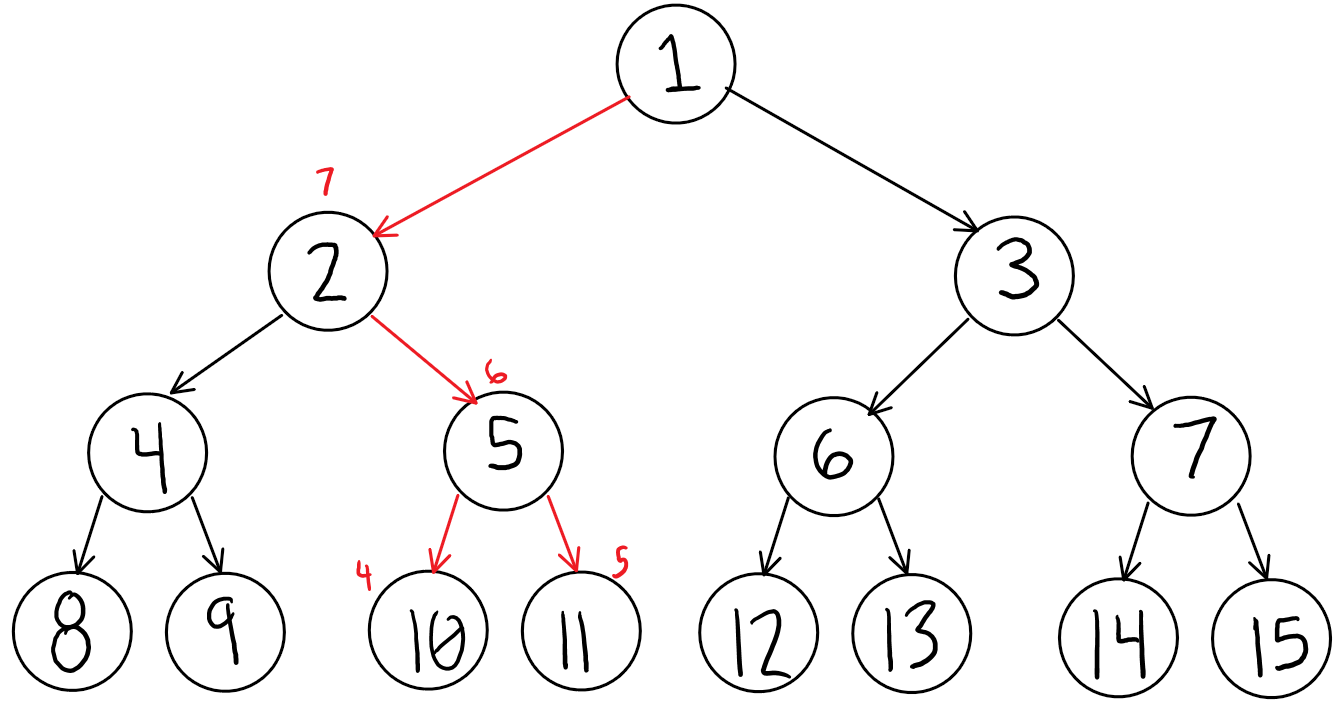
\includegraphics[scale=0.5]{DLS_2.png}
				\caption{Second stage of Depth Limited Search.}
				\label{fig.bfs}
			\end{figure}
			\begin{figure}
				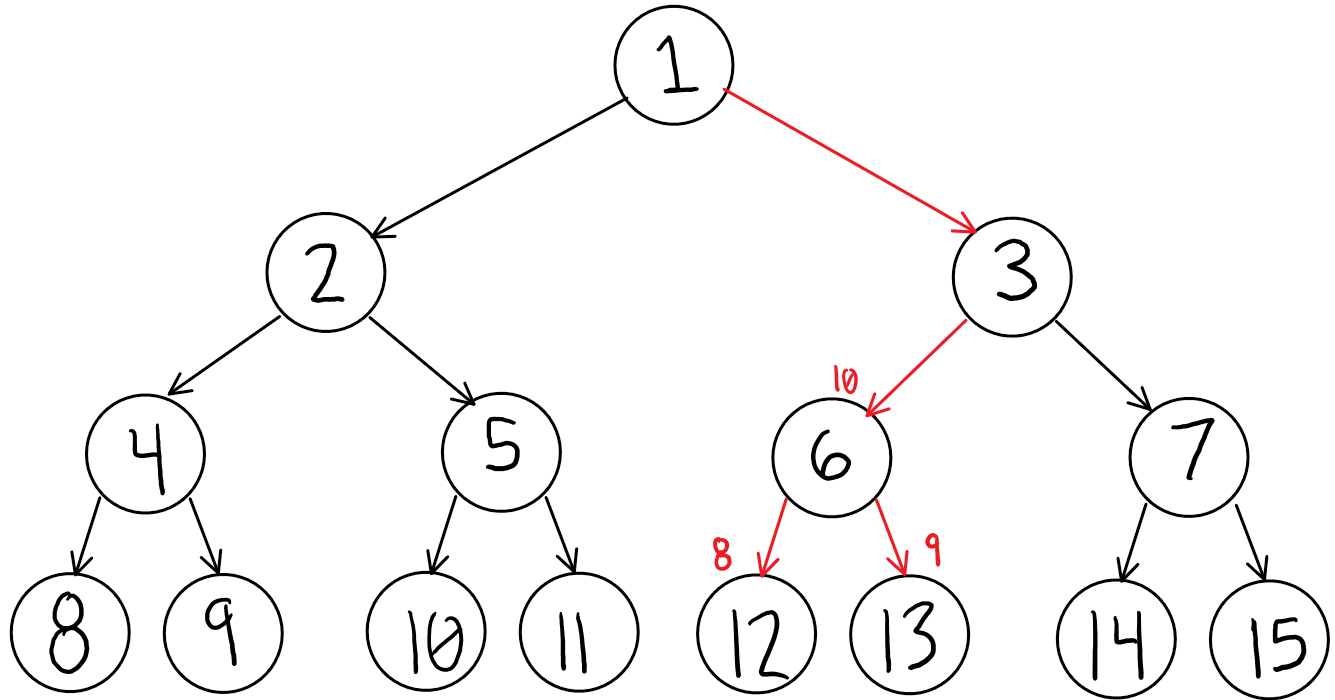
\includegraphics[scale=0.5]{DLS_3.PNG}
				\caption{Third stage of Depth Limited Search.}
				\label{fig.bfs}
			\end{figure}
			\begin{figure}
				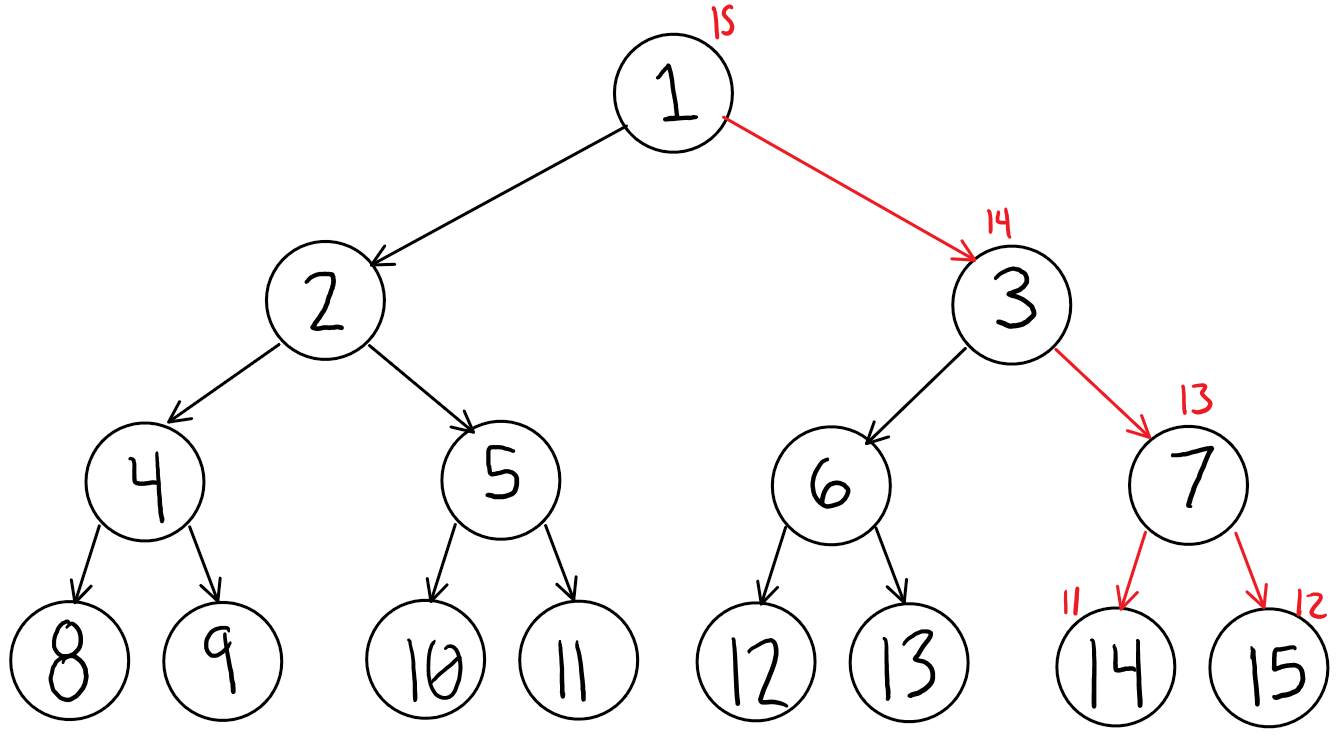
\includegraphics[scale=0.5]{DLS_4.PNG}
				\caption{Final stage of Depth Limited Search.}
				\label{fig.bfs}
			\end{figure}
			\newline
			\begin{large}Iterative Deepening Search\end{large}
			\begin{figure}
				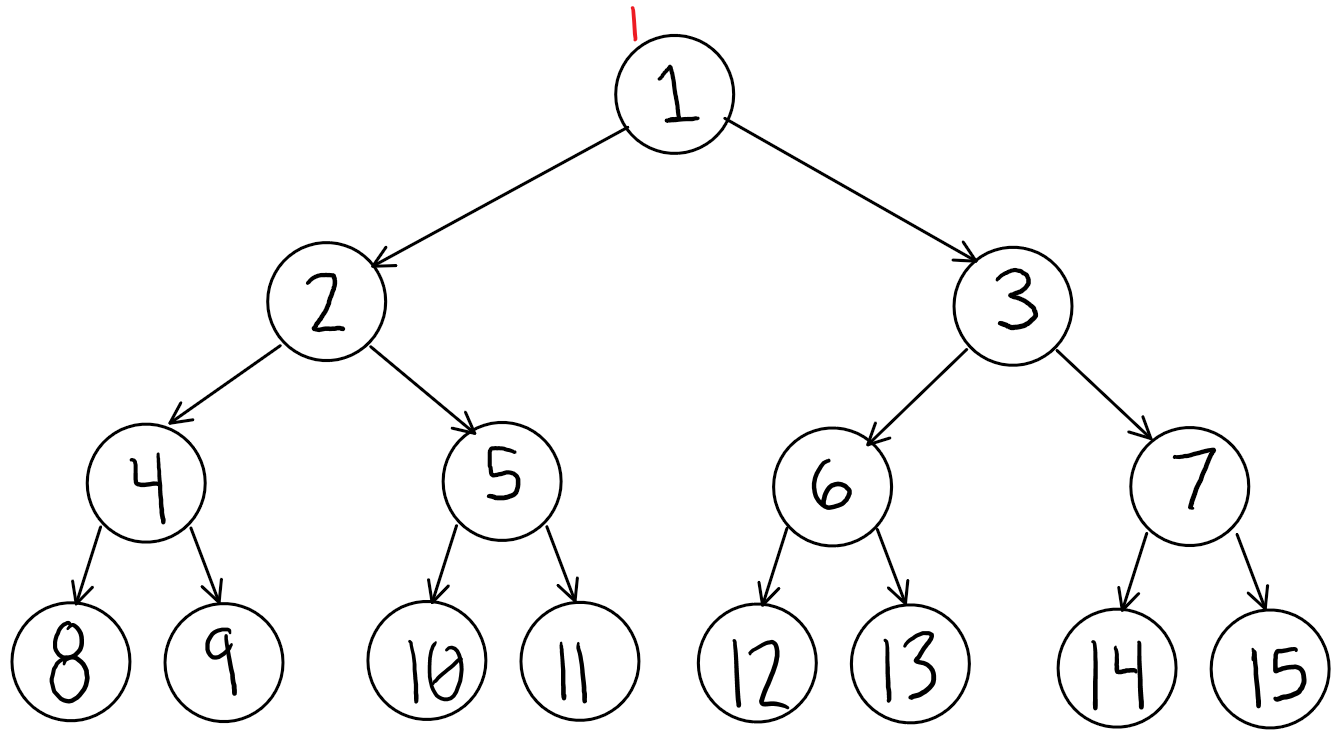
\includegraphics[scale=0.5]{ID_1.PNG}
				\caption{First stage of Iterative Deepening Search.}
				\label{fig.bfs}
			\end{figure}
			\begin{figure}
				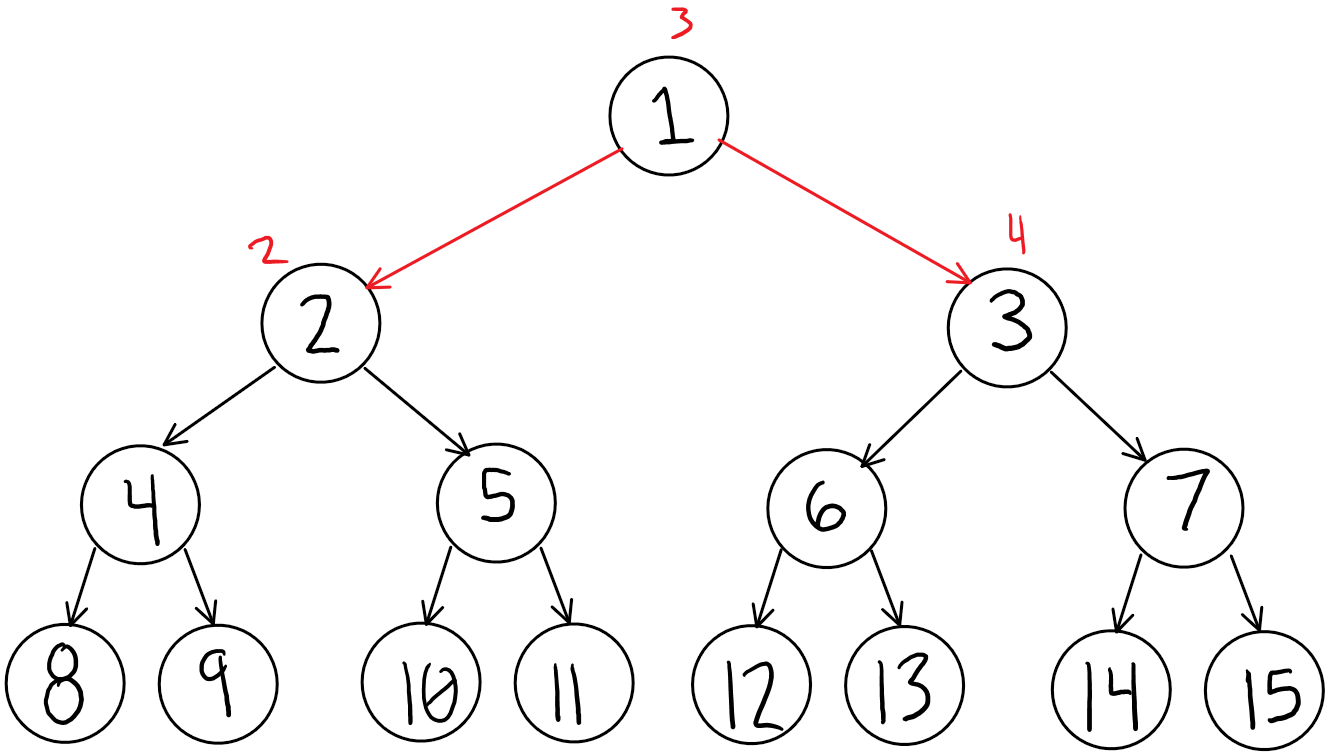
\includegraphics[scale=0.5]{ID_2.PNG}
				\caption{Second stage of Iterative Deepening Search.}
				\label{fig.bfs}
			\end{figure}
			\begin{figure}
				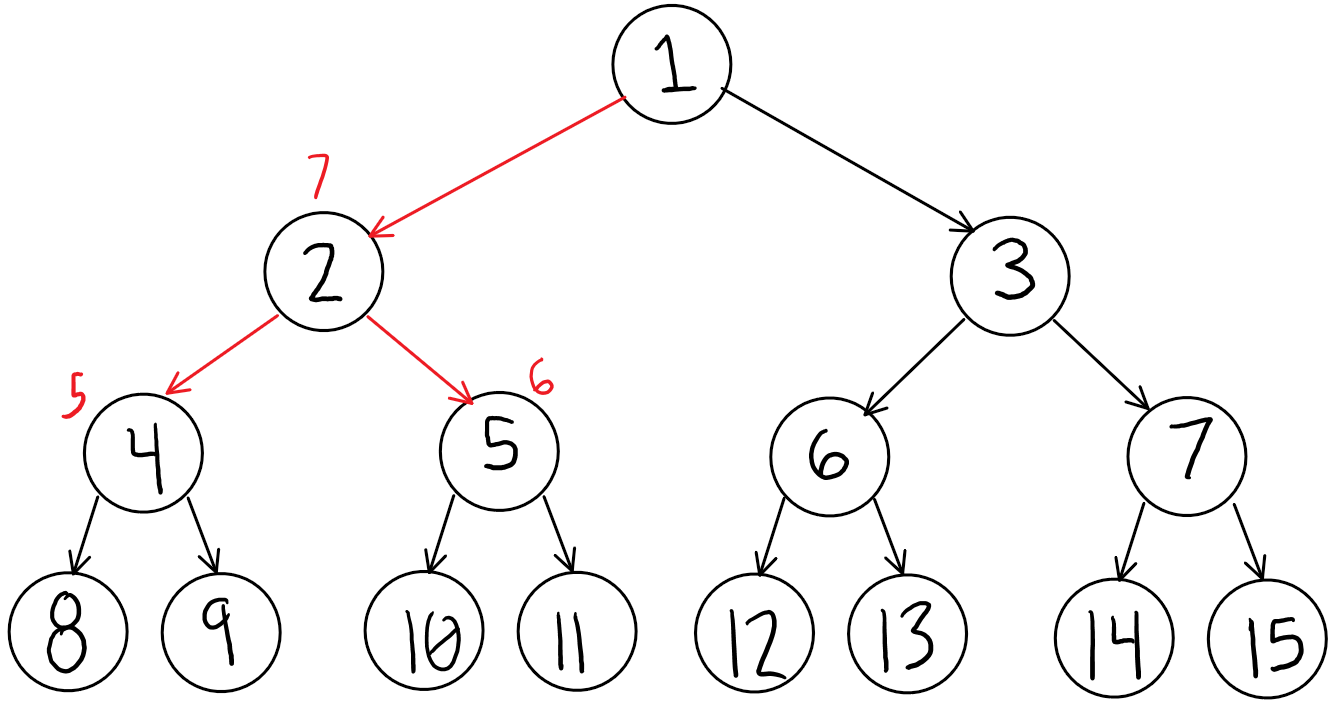
\includegraphics[scale=0.5]{ID_3.PNG}
				\caption{Third stage of Iterative Deepening Search.}
				\label{fig.bfs}
			\end{figure}
			\begin{figure}
				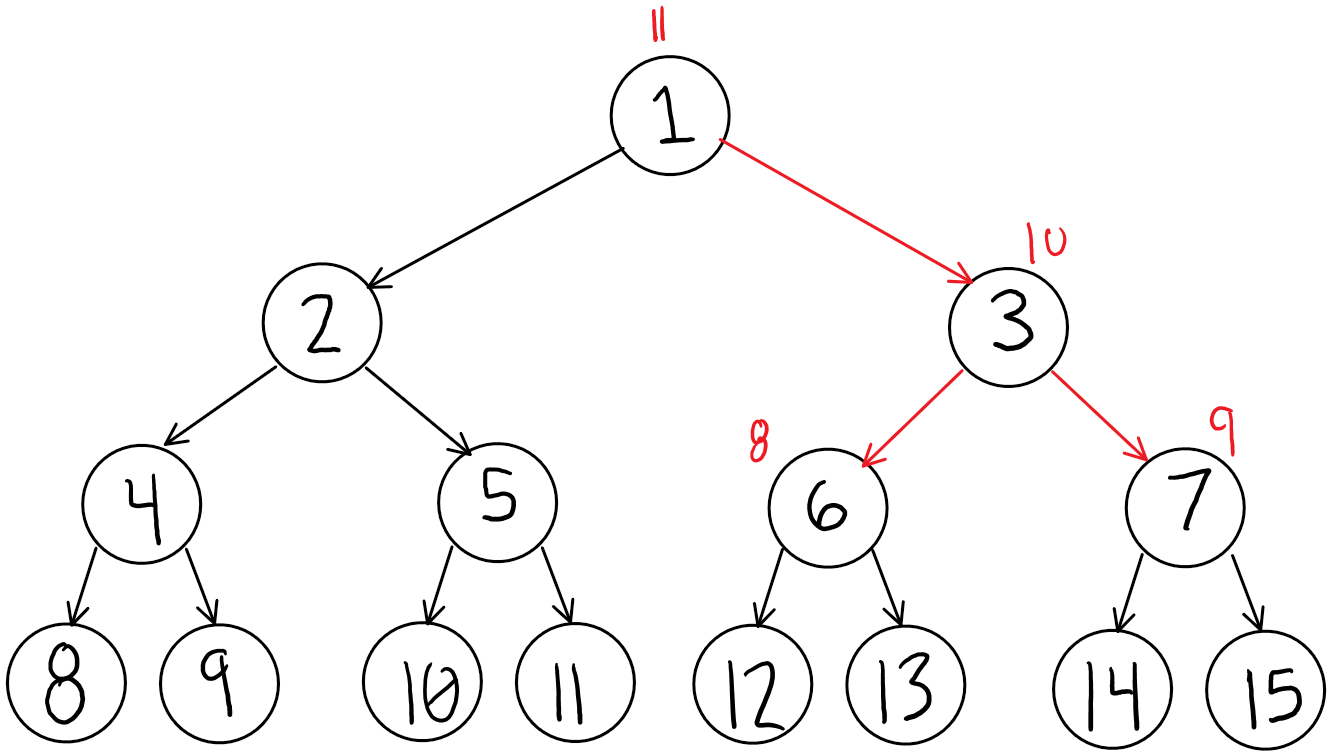
\includegraphics[scale=0.5]{ID_4.PNG}
				\caption{Fourth stage of Iterative Deepening Search.}
				\label{fig.bfs}
			\end{figure}
			\begin{figure}
				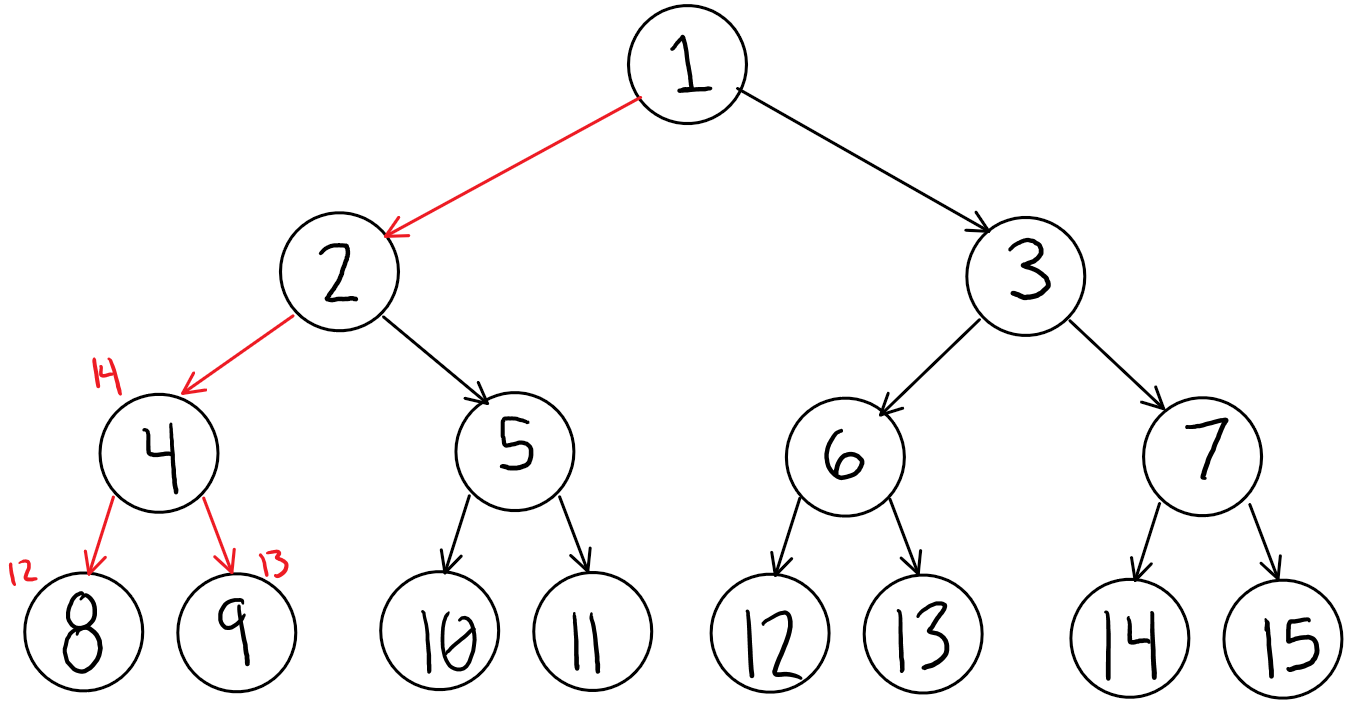
\includegraphics[scale=0.5]{ID_5.PNG}
				\caption{Fifth stage of Iterative Deepening Search.}
				\label{fig.bfs}
			\end{figure}
			\begin{figure}
				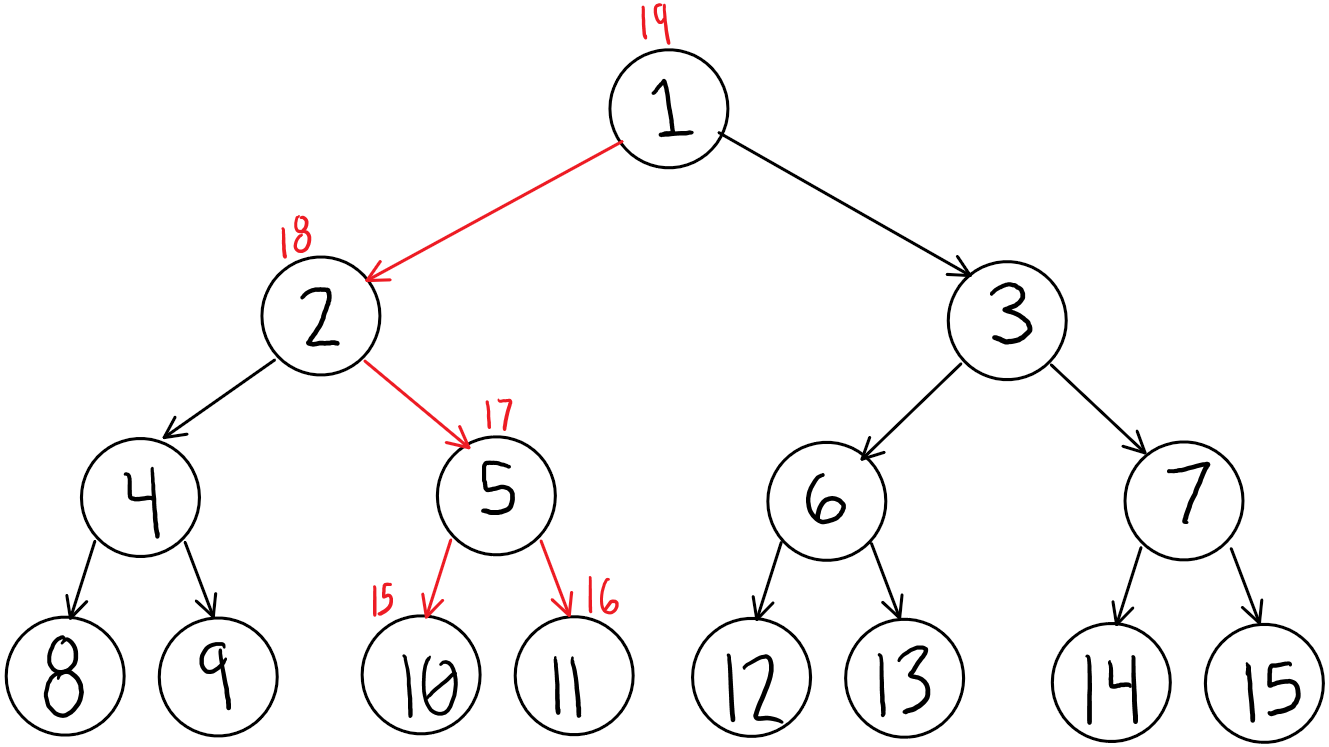
\includegraphics[scale=0.5]{ID_6.PNG}
				\caption{Sixth stage of Iterative Deepening Search.}
				\label{fig.bfs}
			\end{figure}
			\begin{figure}
				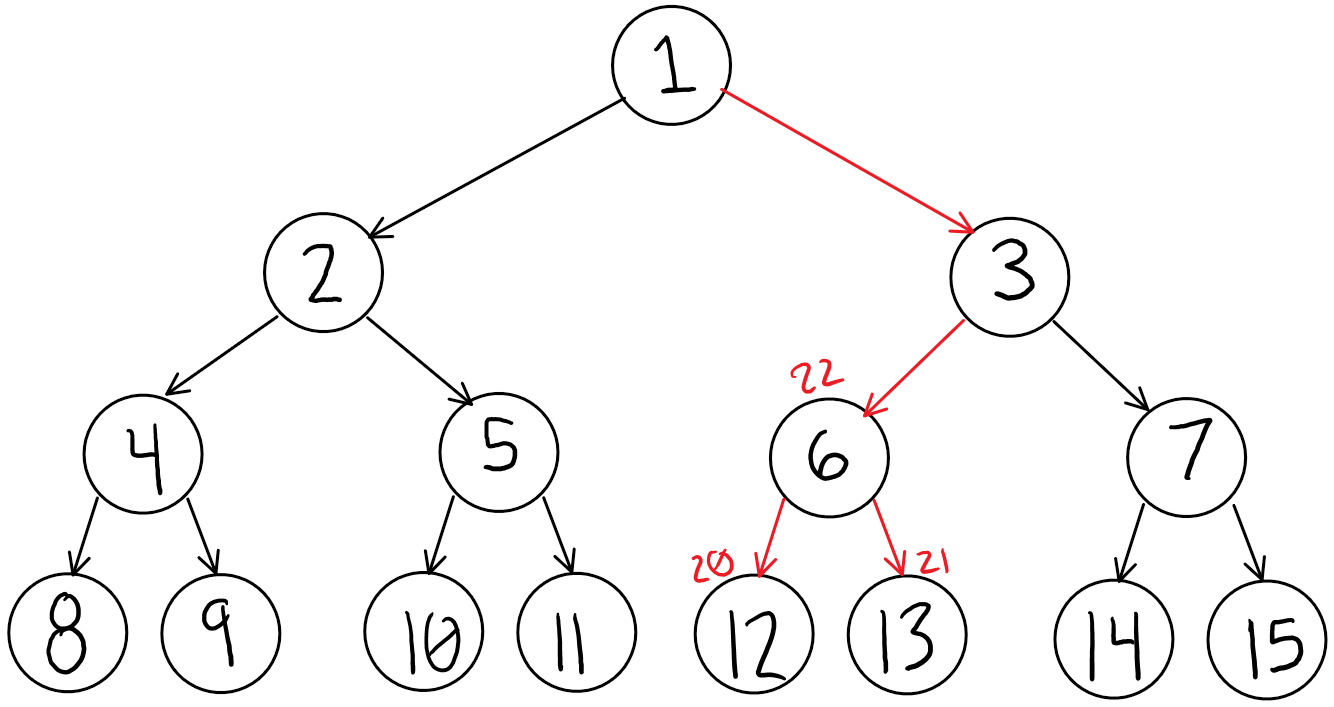
\includegraphics[scale=0.5]{ID_7.PNG}
				\caption{Seventh stage of Iterative Deepening Search.}
				\label{fig.bfs}
			\end{figure}
			\begin{figure}
				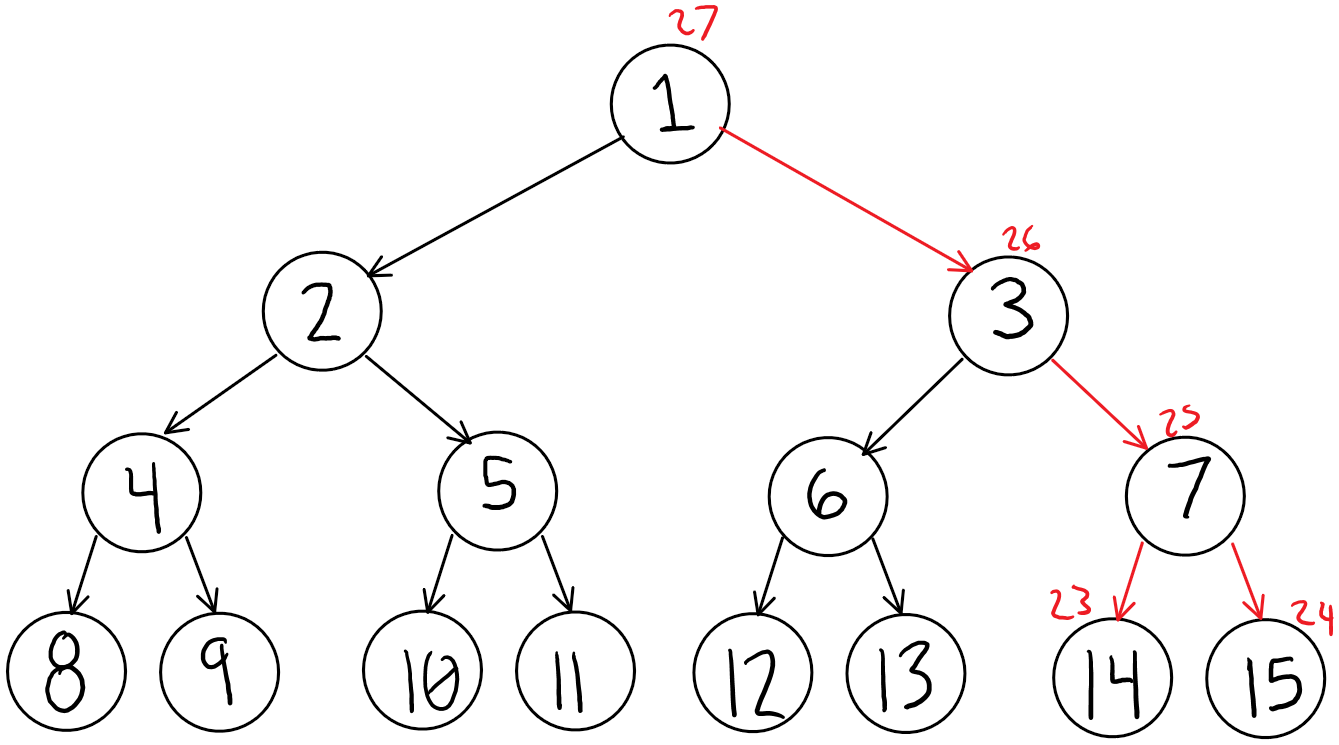
\includegraphics[scale=0.5]{ID_8.PNG}
				\caption{Final stage of Iterative Deepening Search.}
				\label{fig.bfs}
			\end{figure}
		\item Would bidirectional search be appropriate for this problem? If so, describe in detail how it would work. What is the branching factor in the forward and reverse directions?
			\begin{verse}
				A birectional search would be valid for this search, so long as the state transitions can be read in both directions. That is, if node two encodes both its edges to node four and five and its edge back to node one. The search would do a search of depth one from node one, followed by a search of one depth to from node eleven. This process would repeat back and forth until the target is found. In a depth first search, all fifteen nodes would have be expanded before node eleven was found. In iterative deepening and depth limited, this would require twenty and eight nodes to be expanded respectively. For a bidirectional search, however, node one would be expanded along with nodes two and three. Node eleven would be expanded with nodes five. Finally, node two would expand nodes four and five with three expanding nodes six and seven for a total of eight nodes expanded. A standard graph search operates in $O\left(b^d\right)$, where d is the depth and b is the branching factor. A bidirectional stearch, however, reduces the depth to half for two separate paths, reducing the complexity to $O\left(2b^\frac{d}{2}\right)$. In this case, since our branching factor is 2, this results in a total time complexity of $O\left(b^{\frac{d}{2}+1}\right)$.
			\end{verse}
		\item Does the answer to (c) suggest a reformulation of the problem that would allow you to solve the problem of getting from state 1 to a given goal state with almost no search?
			\begin{verse}
				Performing a reverse search from the goal node will give the direct path, in reverse, from the start node. This is because each node in the tree only has one parent, so moving backwards from 11 returns node 5, whose parent is node 2, and finally node 1. For this to be possible with a standard search each node must encode not only its successors but its predecessors.
				Since the transitions follow a specific, defined rule set it is possible to traverse the tree backwards with only mathematical operations. By this method, starting from our goal node, each node in the path before it is $\lfloor\frac{NODE}{2}\rfloor$. In our example, our path from node eleven would be derived as $\lfloor\frac{11}{2}\rfloor = 5, \lfloor\frac{5}{2}\rfloor = 2, \lfloor\frac{2}{2}\rfloor = 1$.
			\end{verse}
	\end{enumerate}
\end{problem}
\end{document}
